%\documentclass[twoside,twocolumn,spanish]{article}
\documentclass{article}
\usepackage[T1]{fontenc}
\usepackage[utf8]{inputenc}
\usepackage{graphicx}
\usepackage[spanish]{babel}
\usepackage{amssymb,amsmath,geometry,multicol,spalign,hyperref}
\setlength\columnsep{20pt}
\usepackage[usenames,dvipsnames]{xcolor}
\usepackage{tikz,mathtools}
\usetikzlibrary{angles}
\usepackage{circuitikz}
\usepackage[nointegrals]{wasysym} 
\usepackage{pgfplots}
\pgfplotsset{width=5cm,compat=1.12}
\usepgfplotslibrary{fillbetween}

\title{Cálculo de la constante de recuperación de un muelle}
\author{Andoni Latorre Galarraga \\ \href{mailto:alatorre73@alumno.uned.es}{alatorre73@alumno.uned.es}}
\date{}
\begin{document}

\maketitle
\begin{abstract}
Se calculan experimentalmente las constantes elásticas de varias configuraciones de muelles y luego se comparan con las contantes esperadas a partir de las constantes individuales de los muelles, que también se miden experimentalmente. Finálmente, se calcula la aceleración de la gravedad utilizando un plano inclinado. Ex experimento se desarrolla de acuerdo con los procesos descritos en \cite{web}.
\end{abstract}

\begin{multicols}{2}

\section*{Fundamento Teórico}
\subsection*{Ley de Hooke}
La ley de Hooke predice que si se aplica una fuerza $F$ a un muelle la elongación $x$ es proporcional a dicha fuerza.
$$
F = - k x
$$
Donde la constante de proporcionalidad $k$ es la constante elástica del muelle. Si se suspende una masa $M$ del muelle, aplicando la segunda ley de Newton, se tiene
$$
Ma=-kx \Rightarrow \frac{d^2x}{dt^2} = -\frac{k}{M} x
$$
De la solución de la ecuación diferencial, $C_1\sen(\sqrt{\frac{k}{M}} t) + C_2\cos(\sqrt{\frac{k}{M}} t)$, se deduce el periodo de oscilación, $T$.
$$
T = 2\pi \sqrt{\frac{M}{k}}
$$
Si la masa se ve afectada por dos muelles, estos dos muelles se comportaran como un único muelle con constante elástica $k_e$, el valor de esta constante dependera de como se coloquen los muelles.
\subsubsection*{En serie}
\begin{center}
    \begin{circuitikz}
      \draw (0,1.25) to[spring, l=$k_1$] (0,2.5);
      \draw (0,0) to[spring, l=$k_2$] (0,1.25);
      \draw[fill=gray!40] (-.25,0) rectangle (.25,-.5);
      \node at (0,-0.25) {$M$};
    \end{circuitikz}
    \end{center}
$$
\frac{1}{k_e} = \frac{1}{k_1} + \frac{1}{k_2}
$$
\subsubsection*{En paralelo}
\begin{center}
    \begin{circuitikz}
      \draw (-0.75,0) to[spring, l=$k_1$] (-0.75,1.25);
      \draw (0.75,0) to[spring, l=$k_2$] (0.75,1.25);
      \draw[fill=gray!40] (-1,0) rectangle (1,-.5);
      \node at (0,-0.25) {$M$};
    \end{circuitikz}
    \end{center}
$$
k_e = k_1 + k_2
$$
\subsection*{Plano inclinado}
Si se coloca un objeto sobre un plano inclinado, la componente de la aceleración de la gravedad, $g$, que hace que se delice hacia abajo es $g\sen\theta$ donde $\theta$ es el ángulo del plano inclinado.
\begin{center}
    \begin{tikzpicture}
        \draw[fill=gray!20] (0,0) coordinate (a) -- ({5*cos(30)},{5*sin(30)}) coordinate (b) -- ({5*cos(30)},0) coordinate (c) -- cycle;
        \draw[fill=gray!40] ({3*cos(30)},{3*sin(30)}) -- ({4*cos(30)},{4*sin(30)}) -- ({4*cos(30)-sin(30)},{4*sin(30)+cos(30)}) -- ({3*cos(30)-sin(30)},{3*sin(30)+cos(30)}) -- cycle;
        \pic[draw = gray, angle radius = 10mm]{angle = c--a--b};
        \node at (1.2, 0.4) {$\theta$};
        \draw[-stealth, thick] ({3.5*cos(30)-0.5*sin(30)},{3.5*sin(30)+0.5*cos(30)}) -- ({3.5*cos(30)+0.5*sin(30)},{3.5*sin(30)-0.5*cos(30)})coordinate (gc);
        \draw[-stealth, thick] ({3.5*cos(30)-0.5*sin(30)},{3.5*sin(30)+0.5*cos(30)}) -- ({3.5*cos(30)-0.5*sin(30)},{3.5*sin(30)-0.75})coordinate (g);
        \draw[-stealth, thick] ({3.5*cos(30)-0.5*sin(30)},{3.5*sin(30)+0.5*cos(30)}) -- ({3.5*cos(30)-1.5*sin(30)},{3.5*sin(30)-0.75+cos(30)}) coordinate (gs);
        \node at (2.72,0.8) {$g$};
        \node at (1.75,1.7) {$g\sen\theta$};
        \node at (3.7,1.2) {$g\cos\theta$};
    \end{tikzpicture}
\end{center}
Suponinedo que el objeto comienza en reposo, la velocidad en un instante $t$ será
$$
v = \int_0^t g\sen\theta dt = tg\sen\theta
$$
Y la distancia recorrida,
$$
x = \int_o^t tg\sen\theta dt = \frac{t^2}{2}g\sen\theta
$$
De donde se tiene:
$$
g\sen\theta = \frac{2x}{t^2}
$$
Tenemos una relación lineal entre $\sen\theta$ y $\frac{2x}{t^2}$ donde la pendiente es $g$.
\section*{Dispositivo Experimental}
El dispositivo experimental consiste en un carril de inclinación variable y un coche que encaja en unas guias en el carril. El carril y el coche tinene lugares donde se pueden unir muelles.
\begin{center}
    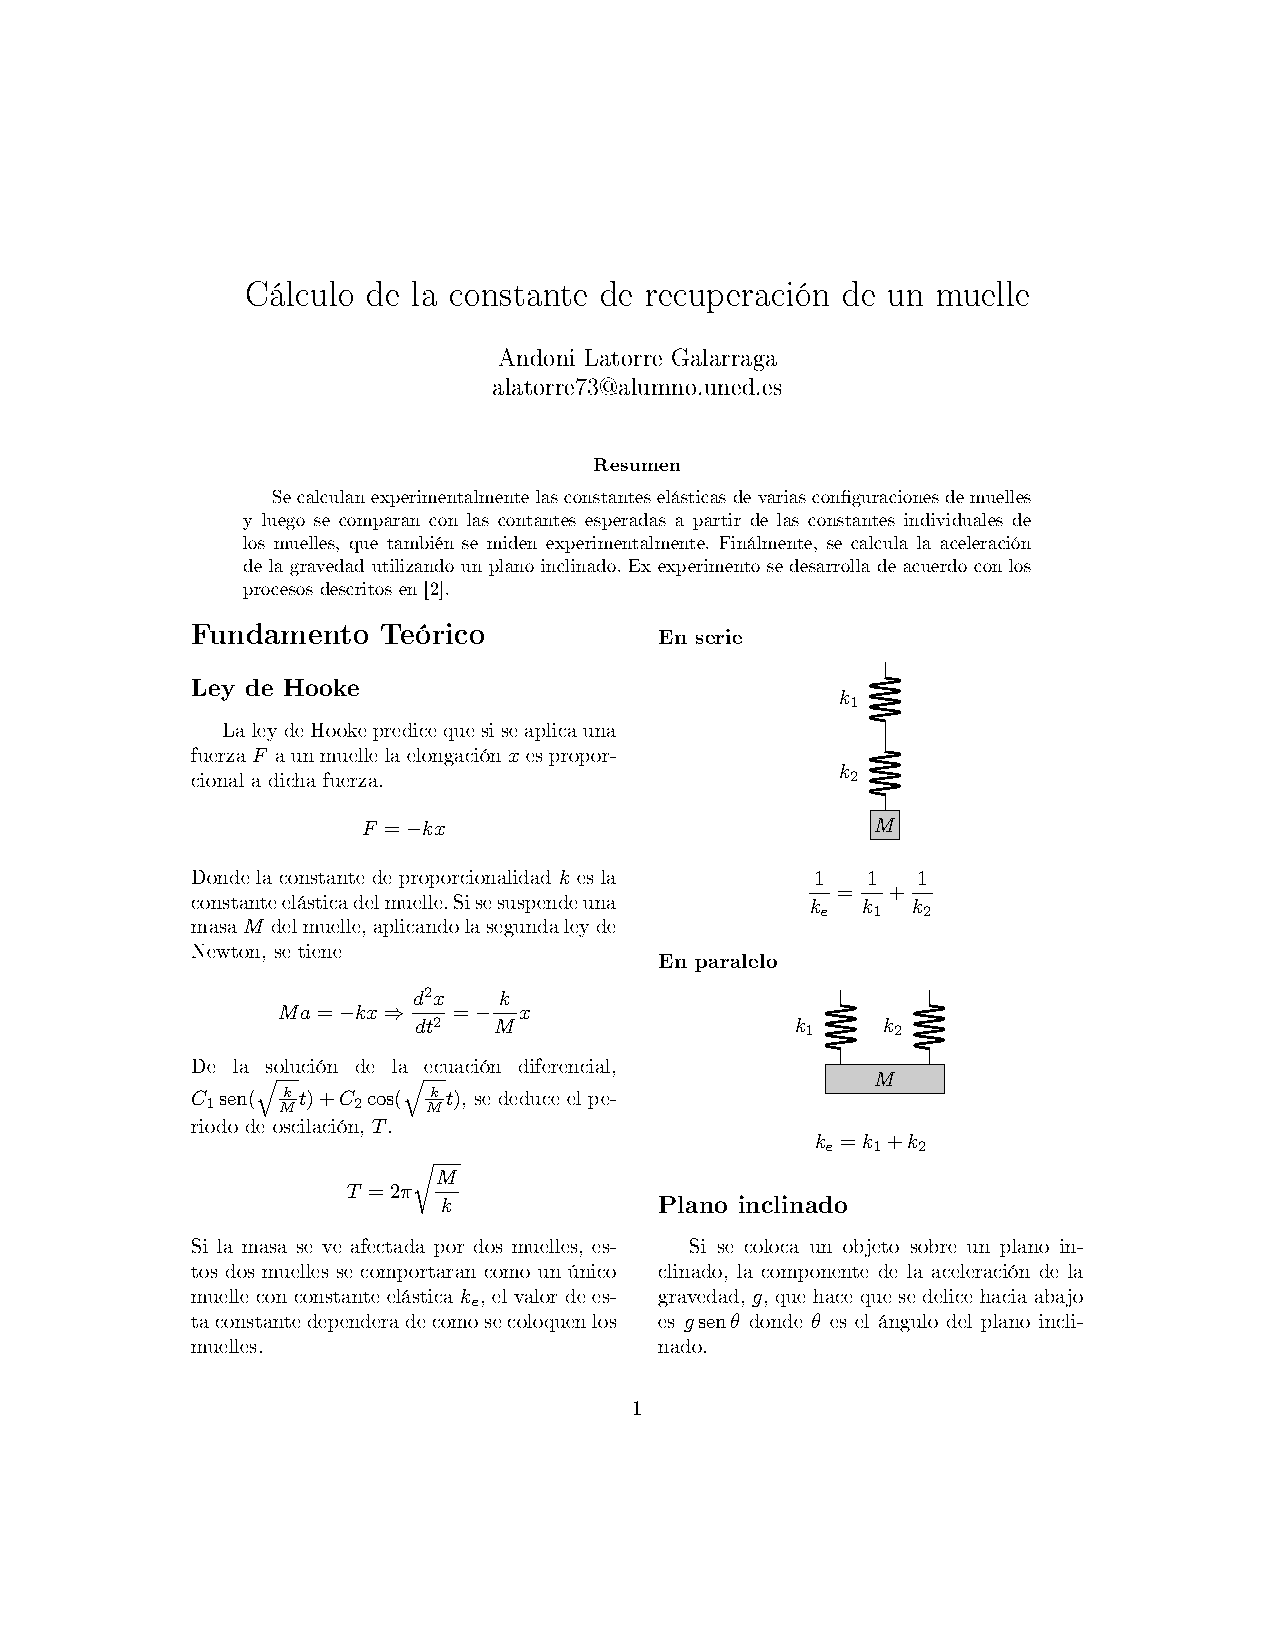
\includegraphics[width=0.45\textwidth]{figures/carril.png}\\
    Figura 1: Coche con un muelle.
\end{center}
El carril también tiene una escala incorporada, con precisión de 1 mm.

\section*{Procedimiento y Resultados}
Primero se ha pesado el coche en dos balanzas, las masas obtenidadas son $(496,2\pm0,1)\text{ g}$ y $(496,4\pm0,1)\text{ g}$. Como la dispersión y la precisión del aparato son iguales tomaremos $0,1$ g como el error y la media como valor esperado de la masa del coche, $m_c$.
$$
m_c = (496,3 \pm 0,1) \text{ g} = (0,4963 \pm 0,001) \text{ kg}
$$
Para dos muelles distintos hemos tomado 5 tiempos distincos correspondientes a 5 coscilaciones cada uno.
\begin{center}
Tabla 1:
$$
\begin{array}{|l||l|l|l|l|l|} \hline
     & T_1\text{(s)} & T_2\text{(s)} & T_3\text{(s)} & T_4\text{(s)} & T_5\text{(s)} \\ \hline \hline
    \text{Muelle 1} & 5.35 & 5.25 & 5.19 & 5.43 & 5.28  \\ \hline
    \text{Muelle 1} & 5.22 & 5.31 & 5.19 & 5.06 & 5.22  \\ \hline
\end{array}
$$
\end{center}
Para el error de cada uno de los tiempos se ha utilizado la dispersión quedando el error de la media, tal como se explica en \cite{manual} p. 45-48.
$$
\overline{T} = \frac{1}{5} \sum_{i=1}^5 T_i \quad D = \frac{\max_i T_i - \min_i T_i}{2}
$$
$$
\epsilon_{\overline{T}} = \frac{D}{\sqrt{5}}
$$
Ahora como, $\overline{T}=5T$ propagando los errores,
$$
T = \frac{1}{5} \overline{T} \quad \epsilon_T = \frac{1}{5} \epsilon_{\overline{T}}
$$
$$
T = \frac{1}{25} \sum_{i=1}^5 T_i \quad \epsilon_T = \frac{\max_i T_i - \min_i T_i}{10\sqrt{5}}
$$
\begin{center}
    Tabla 2:
    $$
    \begin{array}{|l||l|l|} \hline
        & T\text{(s)} & \epsilon_T\text{(s)} \\ \hline \hline
        \text{Muelle 1} & 1.06 & 0.008  \\ \hline
        \text{Muelle 2} & 1.04 & 0.008  \\ \hline
        \end{array}
    $$
\end{center}
Sabiendo la relación entre el periodo y la constante de elasticidad, podemos despejar $k$ y calcualr su error.
$$
k = \frac{4 \pi^2 M}{T^2}
$$
$$
\epsilon_k = \sqrt{
    \left|
        \frac{\partial k}{\partial M}
    \right|^2 \epsilon_M^2
    +
    \left|
        \frac{\partial k}{\partial T}
    \right|^2 \epsilon_T^2
}
$$
$$
= \sqrt{
    \left|
        \frac{4\pi^2}{T^2}
    \right|^2 \epsilon_M^2
    +
    \left|
        -2\frac{4\pi^2 M }{T^3}
    \right|^2 \epsilon_T^2
}
$$
$$
= \frac{4\pi^2}{T^2}\sqrt{
     \epsilon_M^2
    +
    \frac{4M^2}{T^2} \epsilon_T^2
}
$$
\begin{center}
    Tabla 3:
    $$
    \begin{array}{|l||l|l|l|l|} \hline
        & T\text{(s)} & \epsilon_T\text{(s)} & k\text{( kg s\textsuperscript{-2})} & \epsilon_k\text{( kg s\textsuperscript{-2})} \\ \hline \hline
        \text{muelle 1} & 1.06 & 0.008 & 17.4 & 0.3  \\ \hline
        \text{muelle 2} & 1.04 & 0.008 & 18.1 & 0.3  \\ \hline
    \end{array}
    $$
\end{center}
Repetimos este proceso para los muelles en serie (en ambos ordenes) y en paralelo. Los tiempos son los siguentes:
\begin{center}
    Tabla 4:
    $$
    \begin{array}{|l||l|l|l|l|l|} \hline
        & T_1\text{(s)} & T_2\text{(s)} & T_3\text{(s)} & T_4\text{(s)} & T_5\text{(s)} \\ \hline \hline
        \text{Serie 1-2} & 7.78 & 7.71 & 7.91 & 7.97 & 7.75  \\ \hline
        \text{Serie 2-1} & 7.69 & 7.72 & 7.88 & 7.56 & 7.59  \\ \hline
        \text{Paralelo}  & 3.78 & 3.81 & 3.78 & 3.75 & 3.81  \\ \hline
    \end{array}
    $$
\end{center}
Las constantes de elasticidad obtenidas son:
\begin{center}
    Tabla 5:
    $$
    \begin{array}{|l||l|l|l|l|} \hline
        & T\text{(s)} & \epsilon_T\text{(s)} & k\text{( kg s\textsuperscript{-2})} & \epsilon_k\text{( kg s\textsuperscript{-2})} \\ \hline \hline
        \text{muelle 1} & 1.06 & 0.008 & 17.4 & 0.3  \\ \hline
        \text{muelle 2} & 1.04 & 0.008 & 18.1 & 0.3  \\ \hline
        \text{Serie 1-2} & 1.565  & 0.008  & 8.00  & 0.08  \\ \hline
        \text{Serie 2-1} & 1.538  & 0.010  & 8.28  & 0.11  \\ \hline
        \text{Paralelo}  & 0.7572 & 0.0019 & 34.17 & 0.18  \\ \hline
    \end{array}
    $$
\end{center}
Para la segunda parte del experimento, hemos colocado el carril a distintos ángulos y hemos medido el timpo de caida. La distancia recorida por el coche es siempre la misma, $h = (1,100 \pm 0,001)$ m.
\begin{center}
    \begin{tikzpicture}
        \draw[fill=gray!20] (0,0) coordinate (a) -- ({5*cos(30)},{5*sin(30)}) coordinate (b) -- ({5*cos(30)},0) coordinate (c) -- cycle;
        \pic[draw = gray, angle radius = 10mm]{angle = c--a--b};
        \node at (1.2, 0.4) {$\theta$};
        \draw[stealth-stealth] ({-0.25*sin(30)},{0.25*cos(30)}) -- ({5*cos(30)-0.25*sin(30)},{5*sin(30)+0.25*cos(30)});
        \draw[stealth-stealth] ({5*cos(30)+0.25},{5*sin(30)}) -- ({5*cos(30)+0.25},0);
        \node at (2,1.8) {$h$};
        \node at (4.8,1.25) {$x$};
    \end{tikzpicture}
\end{center}
Para calcular $\sen \theta$ mediremos la altura del extremo del carril, $x$. Luego dividiremos entre $h$, la hipotenusa del triangulo. También podemos calcular el error correspondiente.
$$
\sen\theta = \frac{x}{h}
$$
$$
\epsilon_{\sen\theta} = \sqrt{
    \left| \frac{\partial \sen\theta}{\partial h} \right|^2 \epsilon_h^2
    +
    \left| \frac{\partial \sen\theta}{\partial x} \right|^2 \epsilon_x^2
}
$$
$$
=
\frac{1}{h}
\sqrt{
    \frac{4x^2}{h^2} \epsilon_h^2 + \epsilon_x^2
}
$$
$\epsilon_x$ y $\epsilon_h$ son ambos 0,001 m.
$$
\epsilon_{\sen\theta}
=
\frac{0,001}{h}
\sqrt{
    \frac{4x^2}{h^2} +1
}
$$
El experimento se ha realiza poniendo una carga en el coche y sin carga. Los datos son los siguientes:
\begin{center}
    Tabla 6: Sin carga
    $$
    \begin{array}{|l||l|l|l|l|} \hline
        x\text{(m)} & T_1\text(s) & T_2\text(s) & T_3\text(s) & T_4\text(s) \\ \hline \hline
        0.10  & 1.47 & 1.62 & 1.71 & 1.59  \\ \hline
        0.09  & 1.59 & 1.69 & 1.75 & 1.72  \\ \hline
        0.08  & 1.75 & 1.75 & 1.78 & 1.81  \\ \hline
        0.07  & 1.88 & 1.91 & 1.81 & 1.90  \\ \hline
        0.06  & 2.10 & 2.13 & 2.07 & 2.12  \\ \hline
        0.05  & 2.34 & 2.28 & 2.18 & 2.28  \\ \hline
        0.04  & 2.53 & 2.59 & 2.60 & 2.57  \\ \hline
        \end{array}
    $$
    Tabla 7: Con carga
    $$
    \begin{array}{|l||l|l|l|l|} \hline
        x\text{(m)} & T_1\text(s) & T_2\text(s) & T_3\text(s) & T_4\text(s) \\ \hline \hline
        0.10 & 1.47 & 1.41 & 1.50 & 1.56  \\ \hline
        0.09 & 1.64 & 1.75 & 1.75 & 1.69  \\ \hline
        0.08 & 1.82 & 1.75 & 1.78 & 1.82  \\ \hline
        0.07 & 2.00 & 1.96 & 2.00 & 2.03  \\ \hline
        0.06 & 2.16 & 2.07 & 2.09 & 2.09  \\ \hline
        0.05 & 2.34 & 2.34 & 2.21 & 2.28  \\ \hline
        0.04 & 2.59 & 2.63 & 2.69 & 2.53  \\ \hline
    \end{array}
    $$
\end{center}
Calculamos el tiempo medio y su error con las ecuaciondes de \cite{manual} p. 45-48.
$$
T = \frac{1}{4} \sum_{i=1}^4 T_i \quad \epsilon_T = \frac{\max_i T_i - \min_i T_i}{2\sqrt{4}}
$$
\begin{center}
    $$
    \begin{array}{cc}
        \text{Tabla 8: Sin carga} & \text{Tabla 9: Con carga} \\
    \begin{array}{|l||l|l|} \hline
        x\text{(m)} & T\text(s) & \epsilon_T\text(s) \\ \hline \hline
        0.10 & 1.60  & 0.06   \\ \hline
        0.09 & 1.69  & 0.04   \\ \hline
        0.08 & 1.773 & 0.015  \\ \hline
        0.07 & 1.88  & 0.02   \\ \hline
        0.06 & 2.105 & 0.015  \\ \hline
        0.05 & 2.27  & 0.04   \\ \hline
        0.04 & 2.573 & 0.018  \\ \hline
        \end{array}
    &
    \begin{array}{|l||l|l|} \hline
        x\text{(m)} & T\text(s) & \epsilon_T\text(s) \\ \hline \hline
        0.10 & 1.48  & 0.04   \\ \hline
        0.09 & 1.71  & 0.03   \\ \hline
        0.08 & 1.793 & 0.018  \\ \hline
        0.07 & 1.998 & 0.017  \\ \hline
        0.06 & 2.10  & 0.02   \\ \hline
        0.05 & 2.29  & 0.03   \\ \hline
        0.04 & 2.61  & 0.04   \\ \hline
        \end{array}
    \end{array}
    $$
\end{center}
Hemos calculado $\sen\theta$ y su error con las ecuaciones,
$$
\sen\theta = \frac{x}{h} \quad
\epsilon_{\sen\theta}
=
\frac{0,001}{h}
\sqrt{
    \frac{4x^2}{h^2} +1
}
$$
Tambien hemos calculado $\frac{2h}{T^2}$ y su error
$$
 = \sqrt{
    \left|
        \frac{\partial \frac{2h}{T^2}}{\partial h}
    \right|^2 \epsilon_h^2
    +
    \left|
        \frac{\partial \frac{2h}{T^2}}{\partial T}
    \right|^2 \epsilon_T^2
}
$$
$$
 = \frac{2}{T^2}\sqrt{
      \epsilon_h^2
    +
        \frac{4h^2}{T^2}
     \epsilon_T^2
}
$$
\begin{center}
    Tabla 10: Sin carga
    $$
    \begin{array}{|l||l|l|l|} \hline
        \sen\theta & \epsilon_{\sen\theta} & \frac{2h}{T^2} \text{(ms\textsuperscript{-2})} & \epsilon_{\frac{2h}{T^2}} \text{(ms\textsuperscript{-2})} \\ \hline \hline
        0.0909 & 0.0009 & 0.86  & 0.06   \\ \hline
        0.0818 & 0.0009 & 0.77  & 0.04   \\ \hline
        0.0727 & 0.0009 & 0.70  & 0.012  \\ \hline
        0.0636 & 0.0009 & 0.622 & 0.013  \\ \hline
        0.0545 & 0.0009 & 0.496 & 0.007  \\ \hline
        0.0455 & 0.0009 & 0.427 & 0.015  \\ \hline
        0.0364 & 0.0009 & 0.332 & 0.005  \\ \hline
        \end{array}
    $$
    Tabla 11: Con carga
    $$
    \begin{array}{|l||l|l|l|} \hline
        \sen\theta & \epsilon_{\sen\theta} & \frac{2h}{T^2} \text{(ms\textsuperscript{-2})} & \epsilon_{\frac{2h}{T^2}} \text{(ms\textsuperscript{-2})} \\ \hline \hline
        0.0909 & 0.0009 & 1.00  & 0.05   \\ \hline
        0.0818 & 0.0009 & 0.75  & 0.03   \\ \hline
        0.0727 & 0.0009 & 0.684 & 0.014  \\ \hline
        0.0636 & 0.0009 & 0.551 & 0.009  \\ \hline
        0.0545 & 0.0009 & 0.499 & 0.010  \\ \hline
        0.0455 & 0.0009 & 0.420 & 0.011  \\ \hline
        0.0364 & 0.0009 & 0.323 & 0.010  \\ \hline
        \end{array}
    $$
\end{center}
En las siguietes figuras (2 y 3) se puede ver $\frac{2h}{T^2}$ frente $\sen\theta$ con las rectas de regresión cuya pendiente sera nuestra estimación de $g$.
\begin{center}
    \includegraphics[width = 0.45\textwidth]{figures/regresión1.png}\\
    Figura 2: Sin carga. $g = (9.7\pm 0.3) \text{ms\textsuperscript{-2}}$\\
    \includegraphics[width = 0.45\textwidth]{figures/regresión2.png}\\
    Figura 3: Con carga. $g = (11.3\pm 1.2) \text{ms\textsuperscript{-2}}$\\
\end{center}
\section*{Conclusiones}
\subsection*{Costantes elásticas}
Los valores de las constantes de elasticidad, recogidos en la Tabla 5, parecen coincidir con las combinaciones del fundamento teoríco en un a primera observación. Si analicemos detalladamente cada caso.
\subsubsection*{En serie}
Calculamos el error con propagación cuadrática.
$$
k_e = \frac{1}{\frac{1}{k_1} + \frac{1}{k_2}}
$$
$$
\epsilon_{k_e} = \sqrt{
    \left|
        \frac{\partial k}{\partial k_1}
    \right|^2 \epsilon_{k_1}^2
    +
    \left|
        \frac{\partial k}{\partial k_2}
    \right|^2 \epsilon_{k_2}^2
}
$$
$$
\frac{\partial k}{\partial k_1} = \frac{2}{\frac{1}{k_1} + \frac{1}{k_1}} \frac{1}{k_1^2}
$$
$$
\frac{\partial k}{\partial k_2} = \frac{2}{\frac{1}{k_1} + \frac{1}{k_1}} \frac{1}{k_2^2}
$$
$$
\epsilon_{k_e} =
\frac{2}{\frac{1}{k_1} + \frac{1}{k_1}}
\sqrt{\frac{\epsilon_{k_1}^2}{k_1^4} + \frac{\epsilon_{k_2}^2}{k_2^4}}
$$
$$
k_e = (8.87\pm 0.02) \text{ kg s\textsuperscript{-2}}
$$
\subsubsection*{En paralelo}
$$
k_e = k_1 + k_2
$$
$$
\epsilon_{k_e} \sqrt{
    \left|
        \frac{\partial k}{\partial k_1}
    \right|^2 \epsilon_{k_1}^2
    +
    \left|
        \frac{\partial k}{\partial k_2}
    \right|^2 \epsilon_{k_2}^2
}
$$
$$
=
\sqrt{
    \epsilon_{k_1}^2
    +
    \epsilon_{k_2}^2
}
$$
El resultado es:
$$
k_e = (35.5\pm 0.4) \text{ kg s\textsuperscript{-2}}
$$
Los valores obtenidos a partir de las constantes individuales se corresponden con los medidos directamente. Aunque no sean extrictamente compatibles, son suficientemente cercanos como para confirmar las predicciones teóricas.
\subsection*{Plano inclinado}
El valor de la gravedad local se puede consultar en \cite{gravedad} sabiendo que la latitud del laboratorio es de unos $43.3305^\circ$. El valor obtenido en \cite{gravedad} es de $9.8047$ ms\textsuperscript{-2}. De los dos valores el unico que es compatible con el valor real de $g$ es el obtenido sin carga. El valor de $g$ obtenido con carga es incompatible con el valor real y tiene un error relativo superior al 10\% que lo hace poco fiable. Lo más seguro es que que está desviación provenga de lo poco consistente que era el montaje al poner la carga. Al golpear el final del carril, el montaje entero se desplazaba. Pese a haber observado esto durante el experimento e intentar minimizarlo los errores sistematicos procedentes de las sucesivas variaciones del montaje han introducido un gran error en las medidad y han desplazado el valor esperado. Sin embargo, el valor obtenido sin carga es compatible con el valor de \cite{gravedad} y presenta un error del 3\%, un resultado bastante bueno.

\begin{thebibliography}{1}

  \bibitem{manual}Manual de la asignatura. Versión 3.7

  \bibitem{web}\url{https://uned-labo.netlify.app/practicas/te/3_practica_plano_inclinado/prak3.html} 15/6/2022

  \bibitem{gravedad}\url{https://www.sensorsone.com/local-gravity-calculator/} 15/6/2022

\end{thebibliography}
\end{multicols}
\end{document}